\section{Data Analysis Theory}

%\todo{Lägg till overall data table}

%Methods to choose from for analysing (i.e. what I did during the interactions, to test and analyze my app)

%Partly data collection done via app, but also all the observations

The results from each iteration needed to be analysed, using the methods outlined in section \ref{sec:data-analysis}. Depending on the kind of activity and results gathered, different data is collected.

For qualitative methods, the output is almost always observation notes, which are then concluded into insights. These insights, can then sometimes be used in the below analysis methods.

For quantitative data, the output is almost always quiz results or data about the coaches. Before analysis, how this data has been processed is clearly described in chapter \ref{sec:data-analysis}.

Below, an overview of which data analysis method was used for what data is presented. The tools and iteration the tool was used in, is outlined below as a summary:

Qualitative data analysis:
\begin{enumerate}
\item Need groups and Personas (\#1)
\item Customer Journey Map (\#1)
\item Sprint backlog (\#1, \#2, \#3, \#4)
\item Sprint demo (\#1, \#2, \#3, \#4)
\end{enumerate}

Quantitative data analysis:
\begin{enumerate}
\item Correlation in Google Sheets (\#2, \#3, \#4)
\item Correlation in R (\#4)
\item Logistical regression in R (\#4)
\item Parallel coordinates visualisation (\#4)
\end{enumerate}

\subsection{Iteration 1: Uganda Coach Visit}

In iteration 1, the following activities were carried out and then analysed:

\begin{itemize}
\item Stakeholder interview (for Need groups)
\item Coach interview and field visit (for Need groups)
\item Workshop (for Customer Journey Map)
\item Smartphone test (for Need groups)
\end{itemize}

\subsection{Iteration 2: Zambia Coach Training}

In iteration 2, the following activities were carried out and then analysed:

\begin{itemize}
\item App test observations (for Sprint backlog)
\item Quiz results (for Sprint demo)
\item App design workshop: use case 1 (for Sprint backlog)
\item App design workshop: use case 2 (for Need groups)
\end{itemize}

\subsection{Iteration 3: Uganda Formative Test}

In iteration 3, the following activities were carried out and then analysed:

\begin{itemize}
\item App test observations (for Sprint backlog)
\item Service Mini-Sprint - 5 workshops (for Sprint backlog)
\item Field visits (for Sprint demo)
\item Small formative app test (for Sprint backlog)
\item Big formative app test (for Sprint demo)
\end{itemize}

\subsection{Iteration 4: Uganda Summative Test}

In iteration 4, the following activities were carried out and then analysed:

\begin{itemize}
\item Big summative app test (for Sprint demo and quantitative analysis)
\end{itemize}

Data analysis of quiz results were done first by a general overview in Google Sheets, by statistical analysis in R, and by a parallel coordinates visualization. The process to do this, is described below.

\subsection{Analysis Implementation of Quiz Results and Pre-Data}

In this section, the steps needed to analyse the quantitative data is explained in detail, so that others can use a similar approach. In this example, quiz results are from iteration 4, but a similar approach has been taken with the manually recorded quiz results from iteration 2-3 as well.

Data analysis of quiz results was done first by a general overview in Google Sheets, by statistical analysis in R, and by a parallel coordinates visualization. The process to do this is described below.

\subsubsection{Step 1: Data Acquisition from Server}

It was desired to store the data in Google Sheets, thus it was necessary to collect the MongoDB database content, and convert JSON format into a Google Sheets-readable format, like CSV. Multiple approaches were tried, and the Google Chrome extension called Magic Json \citep{agaze} was the one that worked without problems.

\subsubsection{Step 2: Data Acquisition from Pre-Study}

The Pre-study data acquisition was done by instead of looking at the paper-submitted pre-study evaluation forms, using the data processed into Google Sheets.

\subsubsection{Step 3: Data Enhancement of Server Results}

This section presents how data from the server was processed, to enable visualization mapping. To make the data easier to work with, the columns were reordered, and made sortable and filterable. Some columns were given conditional formatting, so it would be easier to spot irregularities, see figure \ref{fig:resultsColored}. After this, some observations could be made.

\begin{figure}[h]
    \centering
    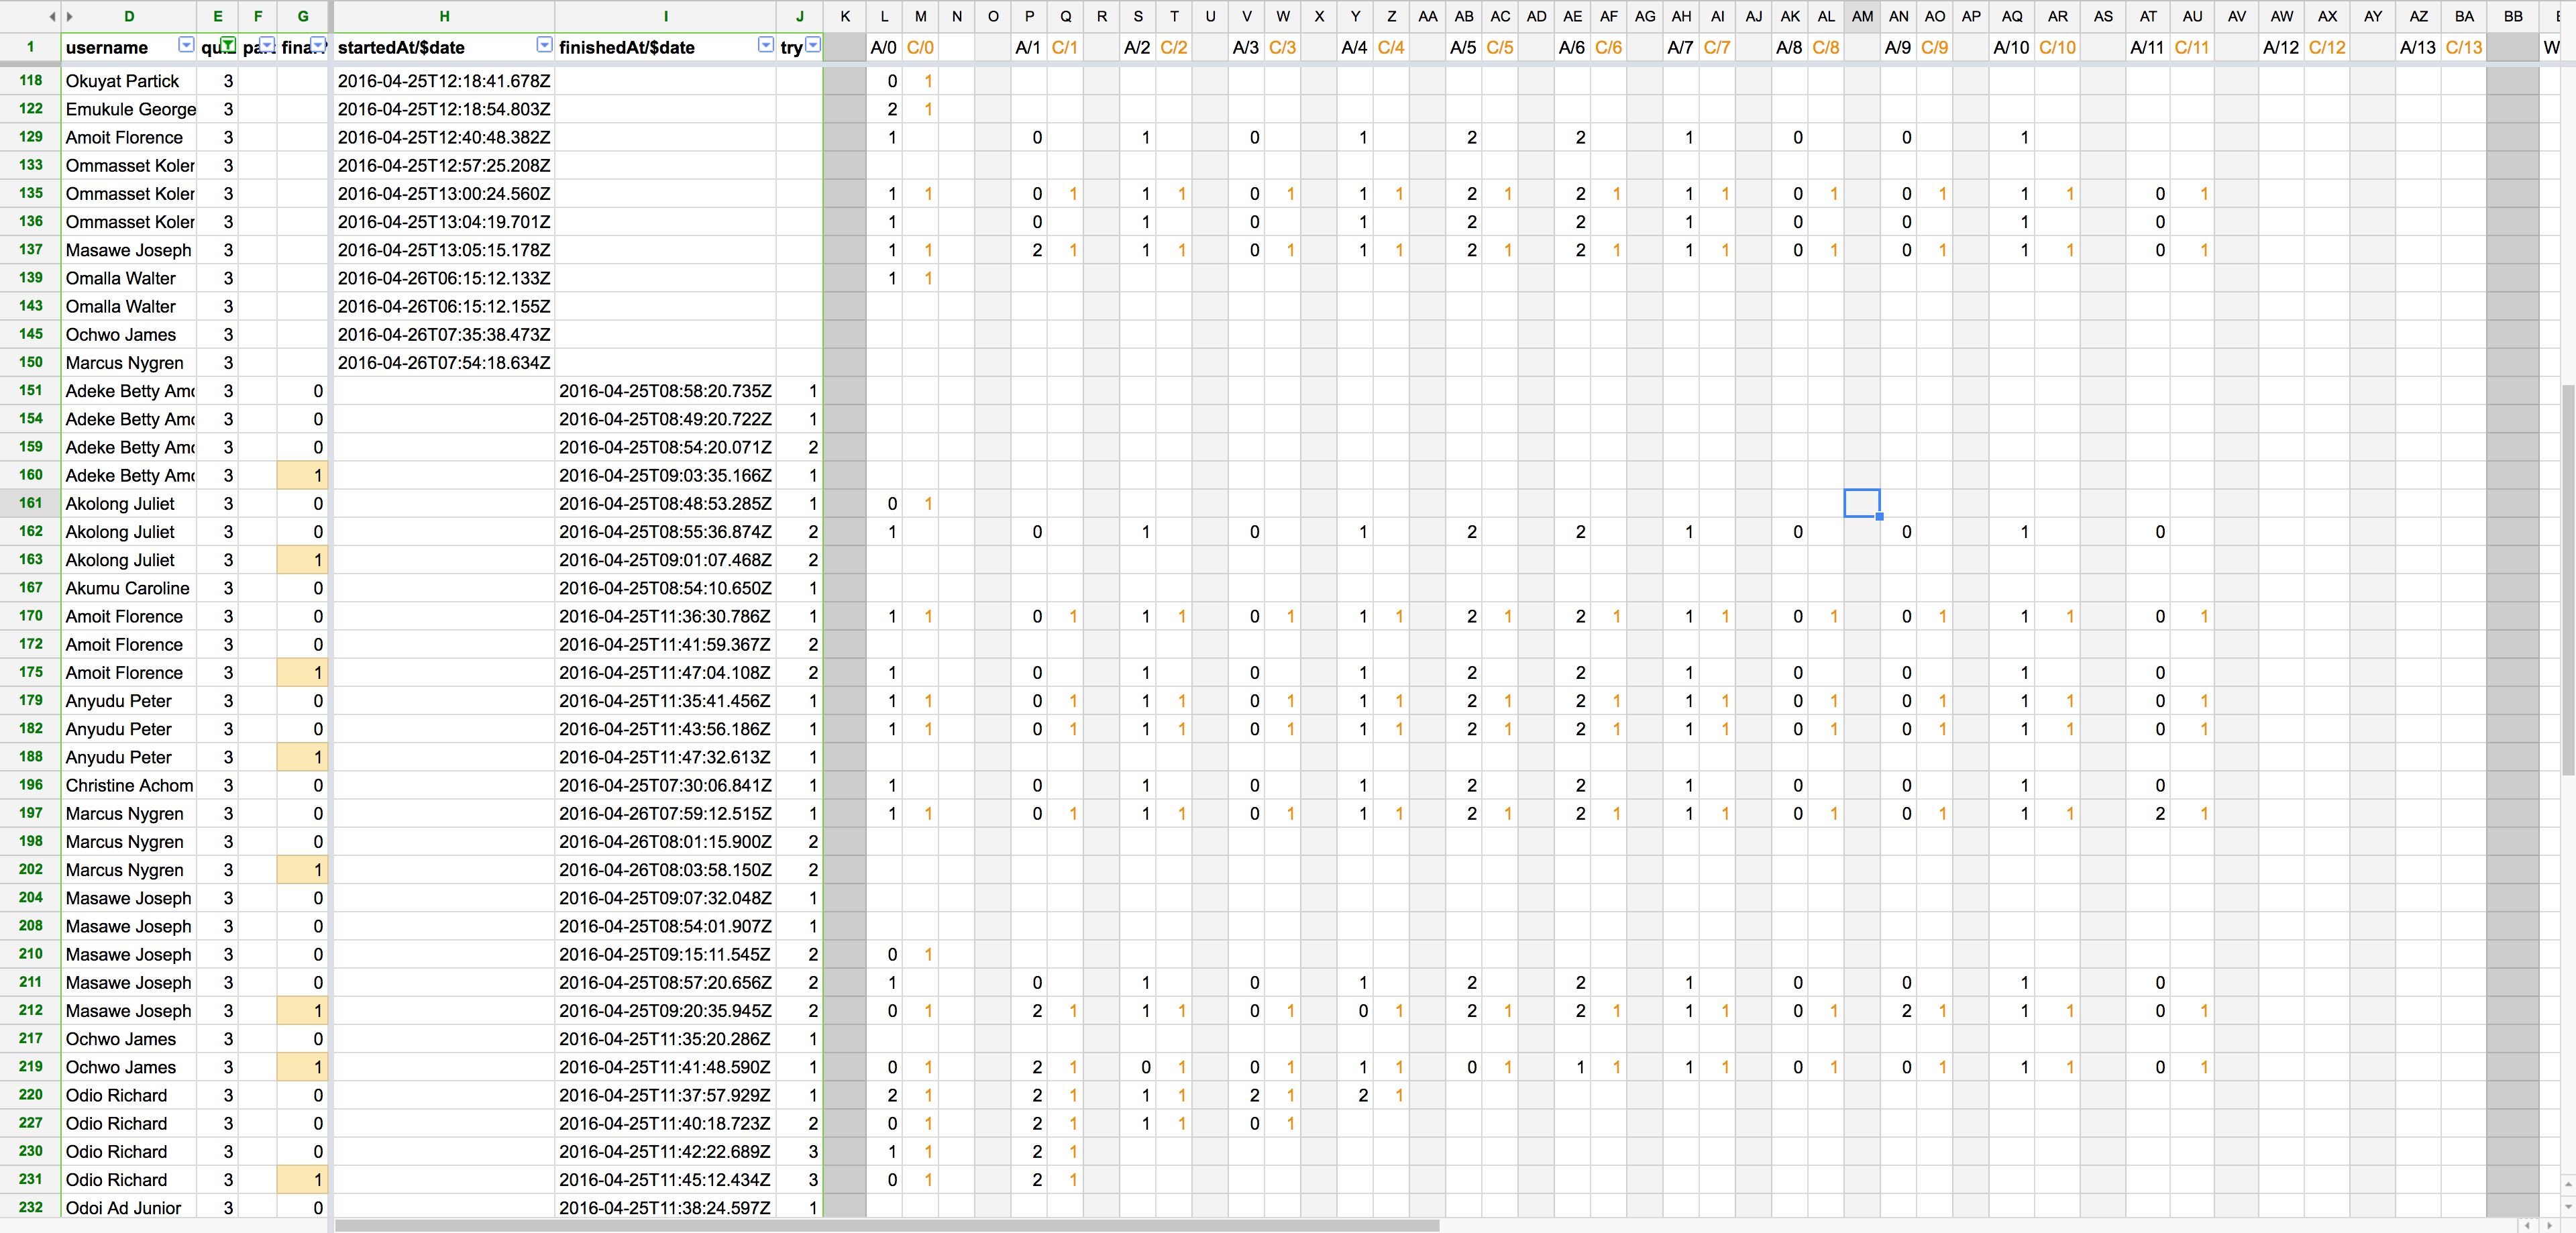
\includegraphics[width=0.9\textwidth]{analysis/resultsColored.png}
    \caption{The quiz results collected in a Google Sheet after data enhancement. In this figure, cell E1 has been filtered so that only results for quiz 3 are shown. Conditional formatting has been done with row G so that if it is a certification quiz, yellow color is used.}
    \label{fig:resultsColored}
\end{figure}

To be able to compare the test results with the pre-test results, it was clear that it would not be viable to test every dimension against every dimension. Instead, since goals of the app evaluation had been predefined in the following way, the quiz results were summarized into a new sheet so that the following could be derived:

\begin{itemize}
\item \% correct 1st try
\item number of tries until 100\%
\item number of tries until 100\% in 1 try
\end{itemize}

These could be calculated by having columns for:

\begin{itemize}
  \item Quiz 3
  \begin{itemize}
    \item Start time training
    \item \% correct 1st try
    \item number of tries until 100\% in 1 try
    \item Time difference start to end time certification
  \end{itemize}
  \item Quiz 9
  \begin{itemize}
    \item Start time training
    \item \% correct 1st try
    \item Time difference start to end 1st try
    \item Time difference start to passed training
    \item Time difference 1st try to certified
  \end{itemize}
\end{itemize}

Then, to see trends, color scales were again added. With ordinal values, a sequential color scheme is used (for example fastest time, from green to red), and with nominal values (like if they are female or male) where there is no right value, a qualitative color scheme is used. Now it was easier to spot outliers and trends, and giving validation to findings from notes and observations made during interviews, workshops and app tests.

\subsubsection{Step 4: Date Enhancement of Pre-study Results}
To see differences in answers more clearly, the data from the pre-study was made sortable and filterable. Then, the data was resampled for each column that had numerable (sortable) data in text instead of numbers, so for example "The day before" was changed to -1 and "The same day" to 0. In a similar way, school level was divided into four different groups, from 0 to 3, where 0 meant secondary, year unknown, 1 meant lower secondary, 2 meant upper secondary, and 3 meant tertiary.

After this, each column was given conditional formats using a color scale, using Google Sheets built-in functionality. This gave a visual way to quickly get an overview of the pre-test data.

\subsubsection{Step 5: Data Enhancement by Joining Pre-test and Results Summary}

The summary sheet and the pre-quiz sheet were joined, becoming a multiple-variate data set (several dimensions that were to bee compared with several other dimensions), see figure \ref{fig:analysFarg3}. A meeting with the university supervisors was held, so they could further give support in how to properly analyse the data. Since the two control groups showed similar means on the pre-quiz results, the two control groups were determined comparable.

\begin{figure}[h]
    \centering
    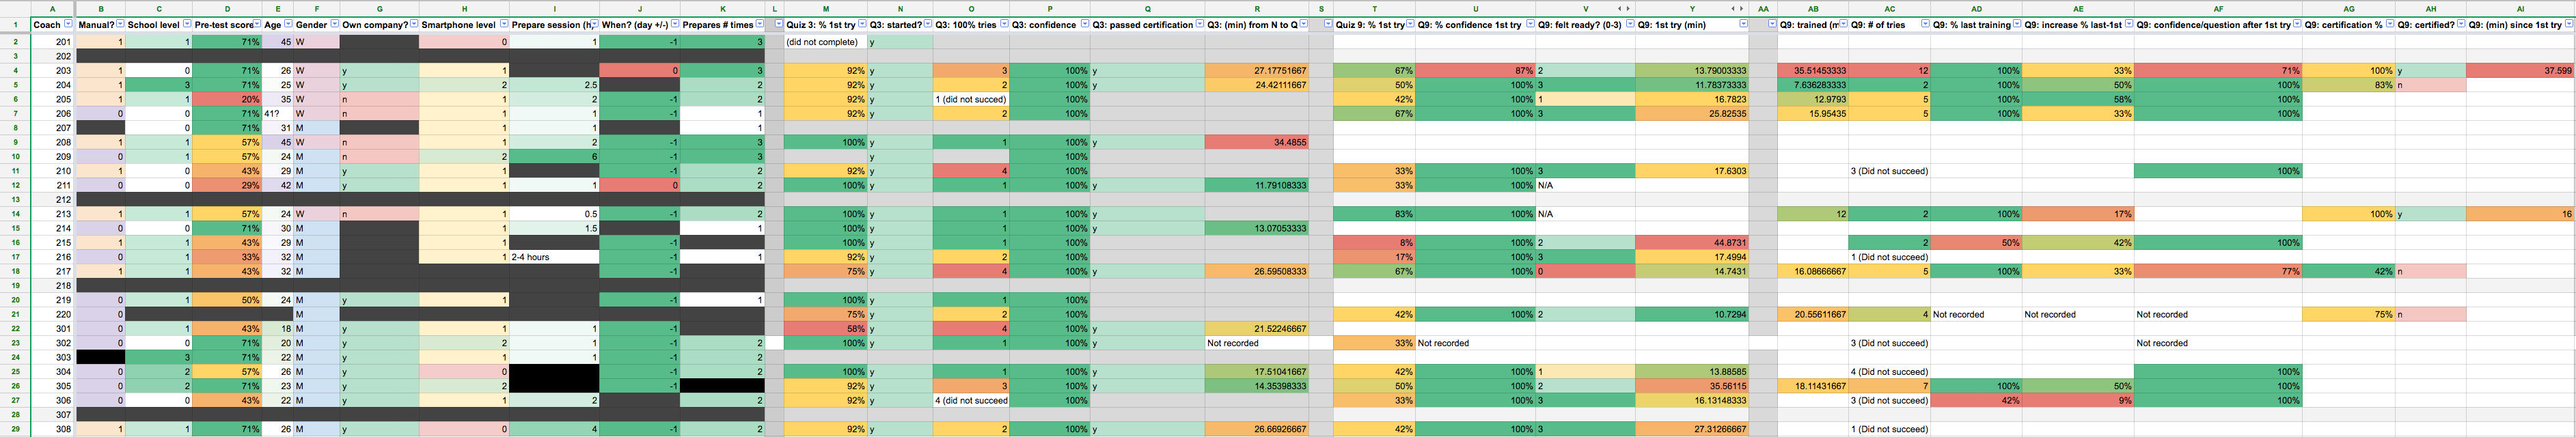
\includegraphics[width=1.0\textwidth]{analysis/sheets/0Overview.png}
    \caption{The multi-variate data set, made filterable and sortable in Google Sheets. Color scales and calculating means makes it easier to compare characteristics of the coach together with pre-test and quiz results. However, it is cumbersome and hard to quickly filter data on multiple parameters.}.
    \label{fig:analysFarg3}
\end{figure}

To meet the challenges of using Google Sheets, a multivariate analyzation software or a visualization was suggested to discover the data in less time. It was hard to determine a suitable multivariate analysis software suitable when having so few data points. Principle Component Analysis or Cohen's kappa would not be suitable, neither was it believed applicable to do Linear correlation on all dimensions. After discussion with other Master thesis students working with analysing data from various disciplines, parallel coordinates was suggested. It would allow very quickly filtering of the data, finding correlations, and distinguish outliers and common characteristics.

To guide the usage of the parallel coordinates (as there is so much to discover in the data set), using R to do Logistic correlation was also done. A disadvantage with this method, is that to be statistically significant, many data points may be needed, and it was now known before-hand if the method would be useful. Probably, parallel coordinates would be the best method to analyse a small multi-variate data set.

\subsubsection{Step 6: Visualization Mapping}
The goal with visualization mapping is to generate renderable data, in this case for the parallel coordinates visualization. Thus, a new spreadsheet is added, specific for visualizing the data. Columns were deleted that would serve no visual purpose (for example timestamps), gave all cells data values (even N/A when undefined), deleting users that did not have data, and shortened the column names so they would fit on the screen. The data was then exported from the Google Sheet into CSV.

\subsubsection{Step 7: Rendering}

For rendering, the JavaScript library D3.js, \citep{d3} was chosen. It supports data-driven documents for visualizing data with HTML, SVG and CSS. It supports both JSON and CSV data. A visual framework for multidimensional detectives for D3.js was found called "Parcoords.js", \cite{parcoords}. The example code from "Linking with a Data Table" provided the basis for the rendering. It allowed observing both the parallel coordinates visualization and the table data from the Google Sheet simultaneously.
% https://syntagmatic.github.io/parallel-coordinates/
% Chang, K. (2012). Parallel Coordinates toolkit : Parcoords.js 0.1. Parallel Coordinates toolkit. Retrieved September 8, 2012, from http://syntagmatic.github.com/parallel-coordinates/
% Kosara, R. (2010, May 13). Parallel Coordinates. Eagereyes.org. Retrieved September 8, 2012, from http://eagereyes.org/techniques/parallel-coordinates
% Tricaud, S. (2008). Picviz: finding a needle in a haystack. Proceedings WASL, San Diego. Retrieved from http://www.usenix.org/events/wasl08/tech/full_papers/tricaud/tricaud.pdf

 %https://syntagmatic.github.io/parallel-coordinates/examples/table.html

To work, the example CSV file was replaced with the data from exporting the Google Sheets data. To benefit the visualization, also the colors were changed, and the toolkit's functionality to drag the axes titles around to reorder the dimensions was used, since the goal was to quickly compare and find correlations. The result is visible in \ref{fig:parallell-coordinates-1}.

\begin{figure}[h]
    \centering
    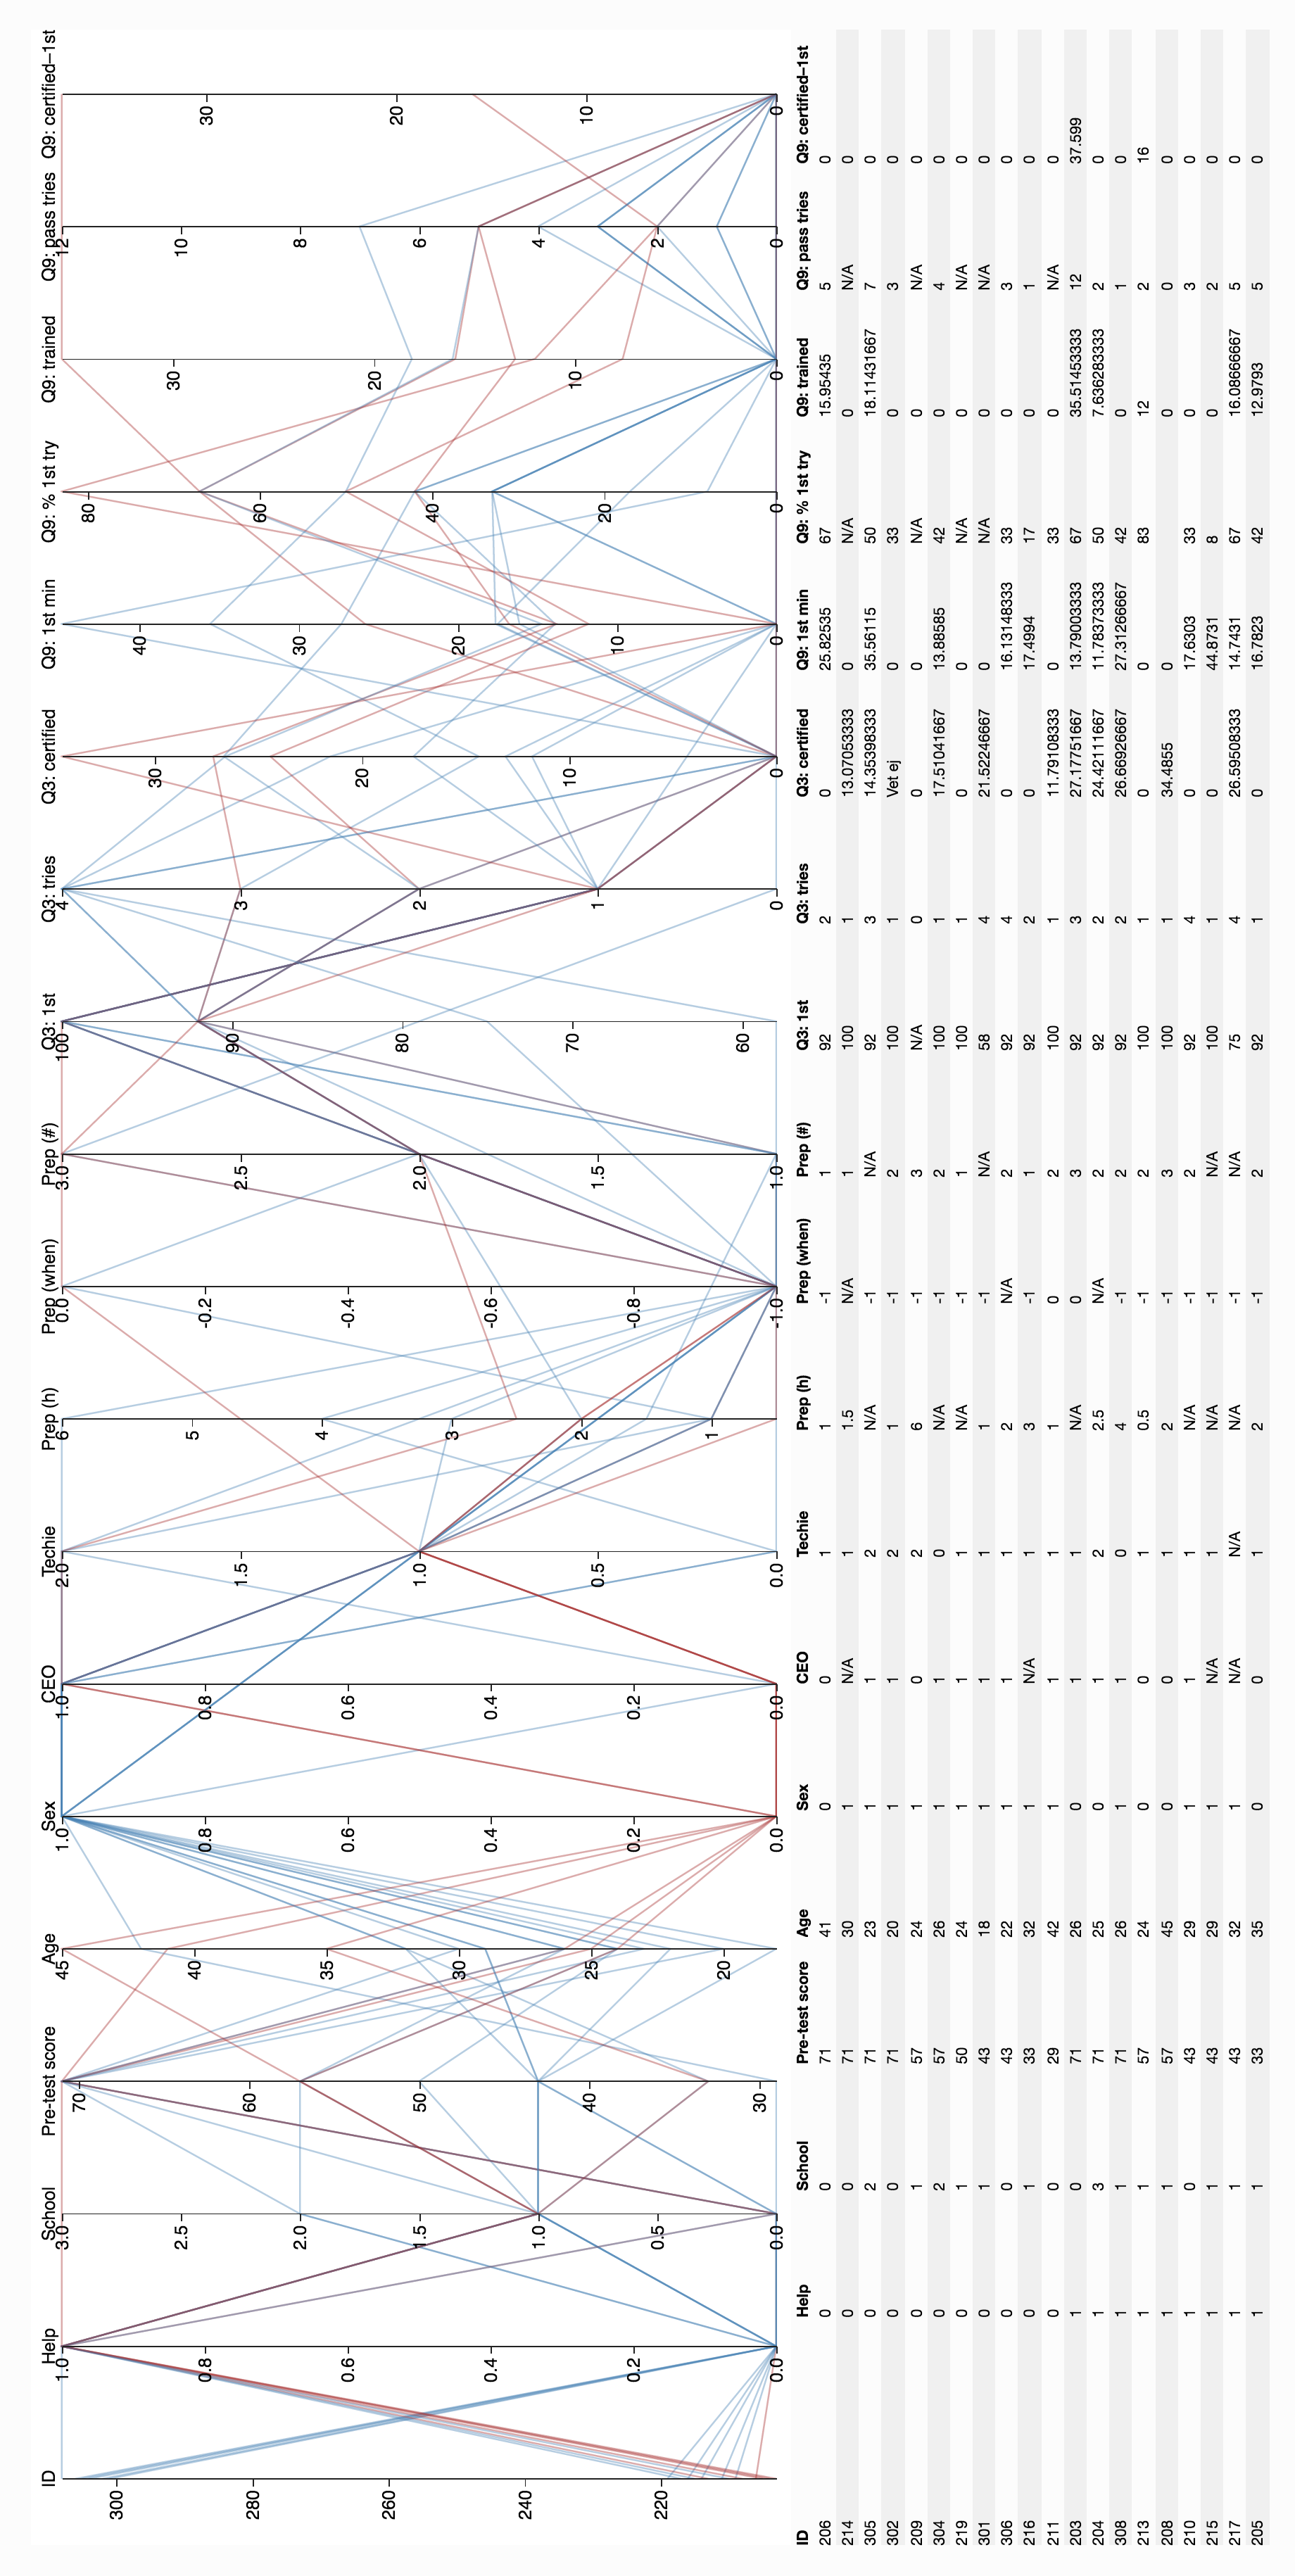
\includegraphics[width=0.7\textwidth]{analysis/parallellCoordinates3.png}
    \caption{The parallel coordinates visualization, done in d3.js. The visualization support draggable axes, filtering of data via dragging the sliders (which synchronizes with the data table), color assignment (like blue and red for men and women in the example), and hovering over a specific data point.}
    \label{fig:parallell-coordinates-1}
\end{figure}

